\newpage
\section{Introduction to injections}
\genHeader
\hypertarget{sec:injections common}{}

This short introducion will show you how to implement small methods by adding handwritten code to classes created from your model. Injections are inspired by
partial classes in C\#, and are our preferred way of providing a clean separation between generated and handwritten code. 

Let's implement the \texttt{removeCard} method declared in the \texttt{Partition} class. All we need to do to `remove' a card from a partition however, is
disable the link between two, but we can't forget that not only does \texttt{removeCard} have to pass in a \texttt{Card}, it must return one as well.

\begin{itemize}


\item[$\blacktriangleright$] Open ``gen/LearningBoxLanguage.impl/PartitionImpl.java'' and enter the following code at the end of the file\footnote{To avoid
errors, you are able to copy/paste this text.}. Do not remove the comment, which is necessary to indicate that this code is written by the user and needs to be
extracted into our injection file.

\begin{figure}[htbp]
        \centering
        \begin{lstlisting}[language=Java, keywordstyle={\bfseries\color{purple}}, backgroundcolor=\color{white}]
    public Card removeCard(Card toBeRemoved) {
        // [user code injected with eMoflon]
        
        toBeRemoved.setCardContainer(null);
        return toBeRemoved;
    }
        \end{lstlisting}
        \caption{Implementation of \texttt{addToStringRep}}
        \label{fig:addToStringRep_impl}
\end{figure}

\item[$\blacktriangleright$] Right-click on Partition.java and choose ``eMoflon/ Create/Update Injection for class'' (Fig.~\ref{fig:injection_create_injection}) 
    
\item[$\blacktriangleright$] This creates a new file in the ``injection'' folder of your project with the same packages and name as the Java class, but with a
new \texttt{.inject} extension (Fig.~\ref{fig:injection_folder}). 

\item[$\blacktriangleright$] Double click to view this file. It contains the definition of a \textit{partial class}~(Fig.~\ref{fig:injection_partialClass}).

\item[$\blacktriangleright$] Save and rebuild your project to complete your handwritten code.

\item[$\blacktriangleright$] While this is a remarkably simple process, it can quickly become challenging when implemented complex functions. Instead, we'll
learn how and continue to implement our method signatures with Story Diagrams in Part III.

\end{itemize}

\clearpage

\vspace*{3cm}

\begin{figure}[htbp]
    \centering
    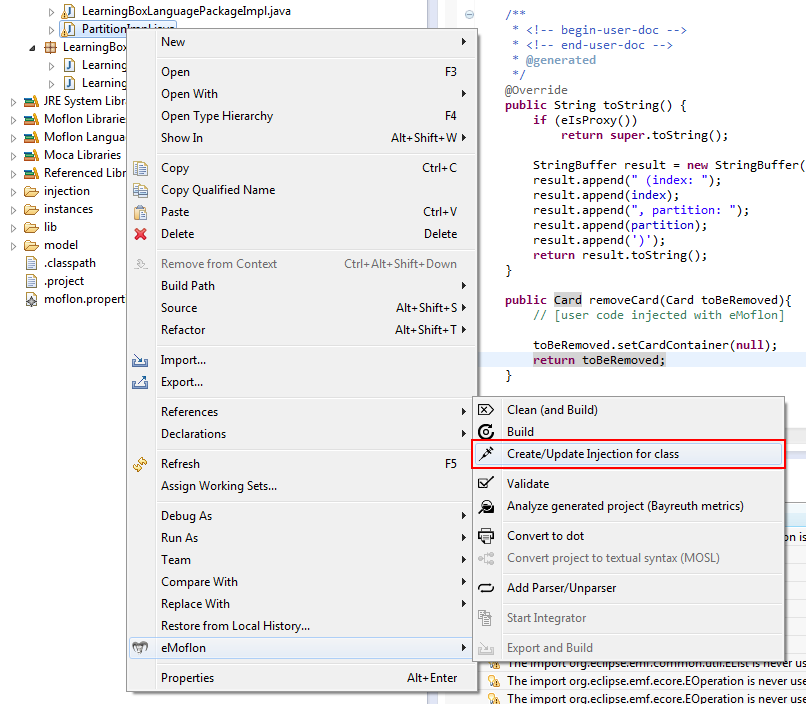
\includegraphics[width=\textwidth]{eclipse_injectionCreate}
    \caption{Create a new injection}
    \label{fig:injection_create_injection}
\end{figure}

\clearpage
\fancyfoot[R]{ $\triangleright$ \hyperlink{sec:LBGUI}{Next}}

\vspace*{0.5cm}

\begin{figure}[htbp]
    \centering
    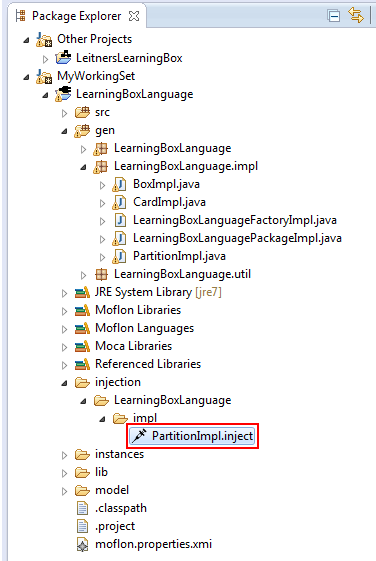
\includegraphics[width=0.5\textwidth]{eclipse_injectionFolder}
    \caption{Injection location}
    \label{fig:injection_folder}
\end{figure}

\vspace{2cm}

\begin{figure}[htbp]
    \centering
    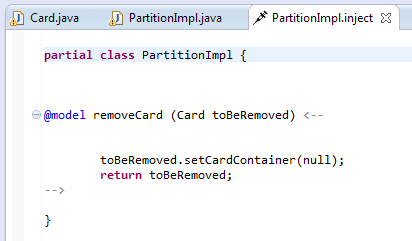
\includegraphics[width=0.5\textwidth]{eclipse_partialClass}
    \caption{Generated Injection file}
    \label{fig:injection_partialClass}
\end{figure}
